\begin{figure*}
	\center
	\begin{subfigure}[b]{0.49\textwidth}
		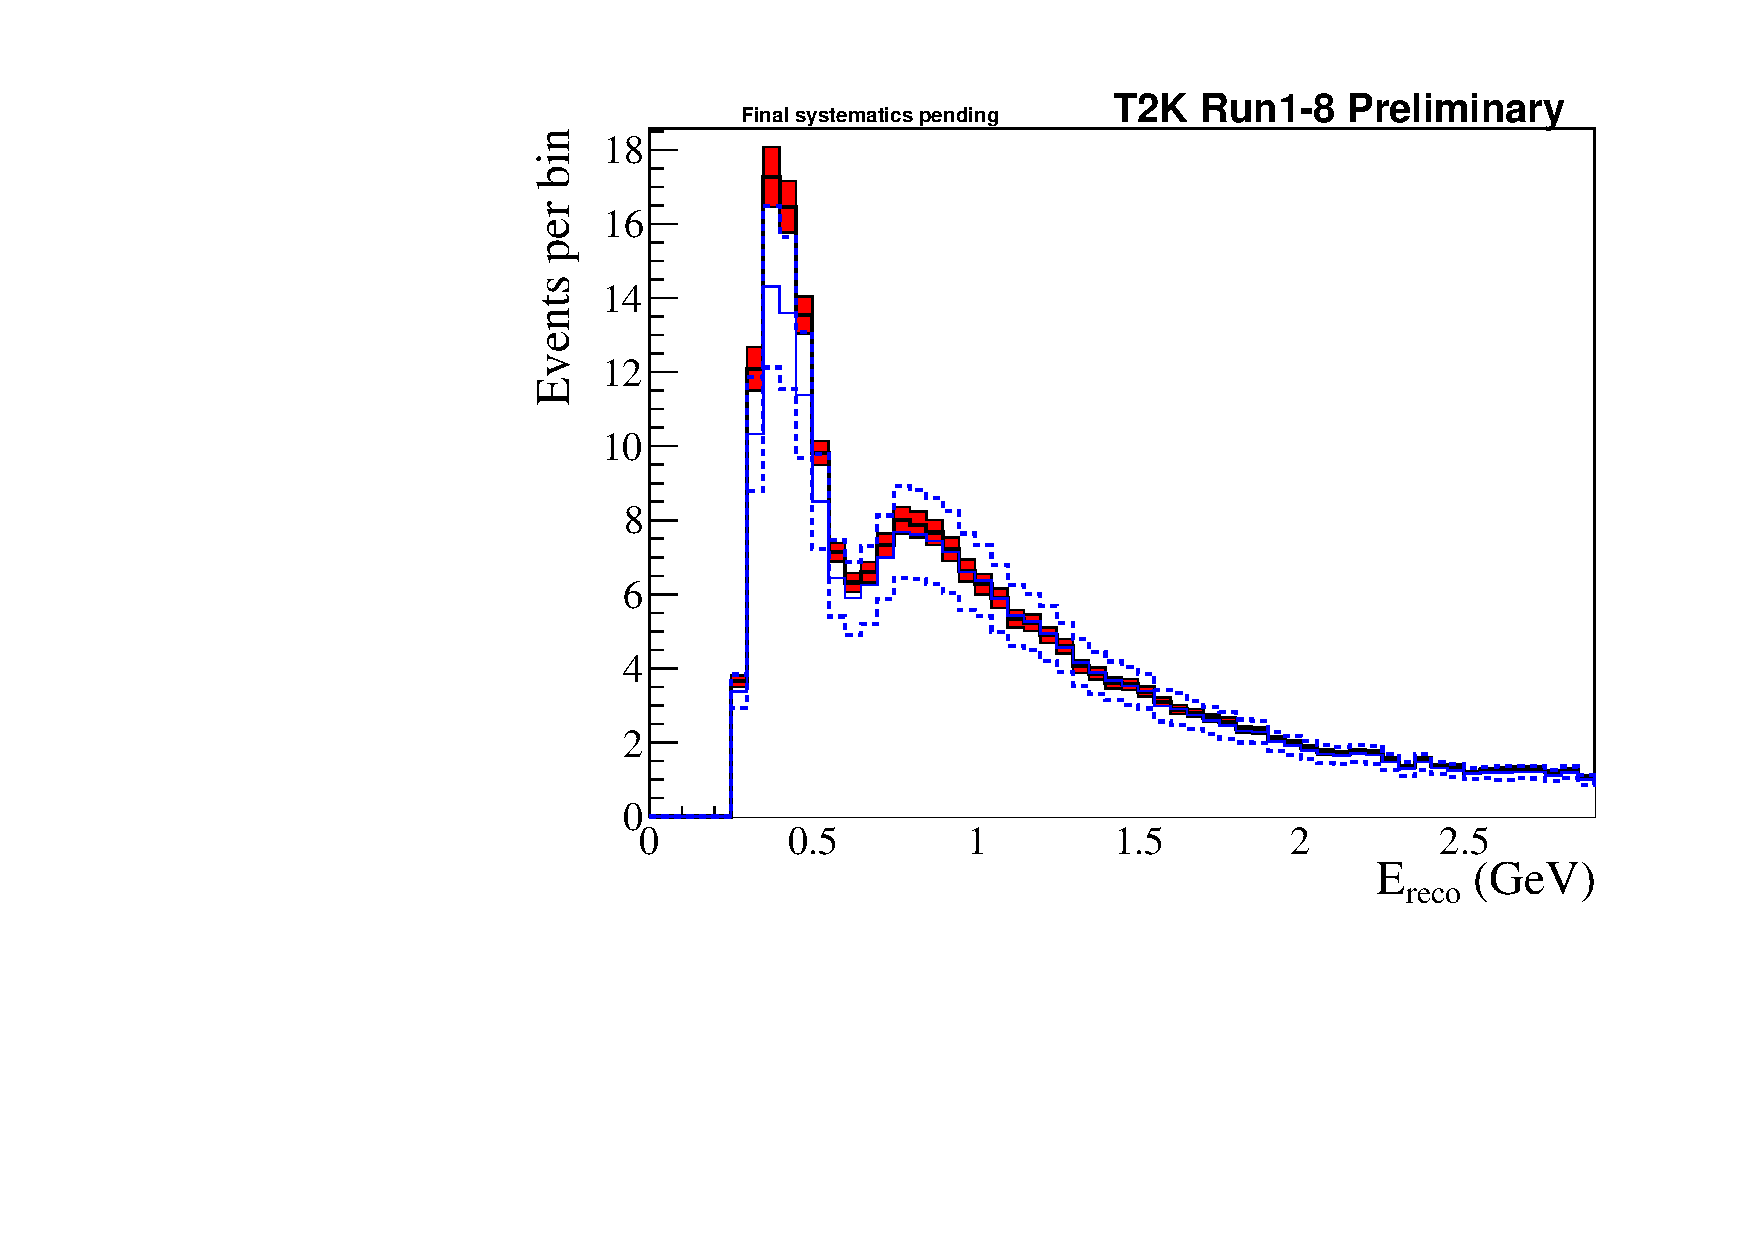
\includegraphics[width=0.9\textwidth]{systematics/envelopes/sk_errors/sk_error_table_1Rmu_banff_constrained_envelope}
		\caption{Muon-like, neutrino mode}
	\end{subfigure}
	\begin{subfigure}[b]{0.49\textwidth}
		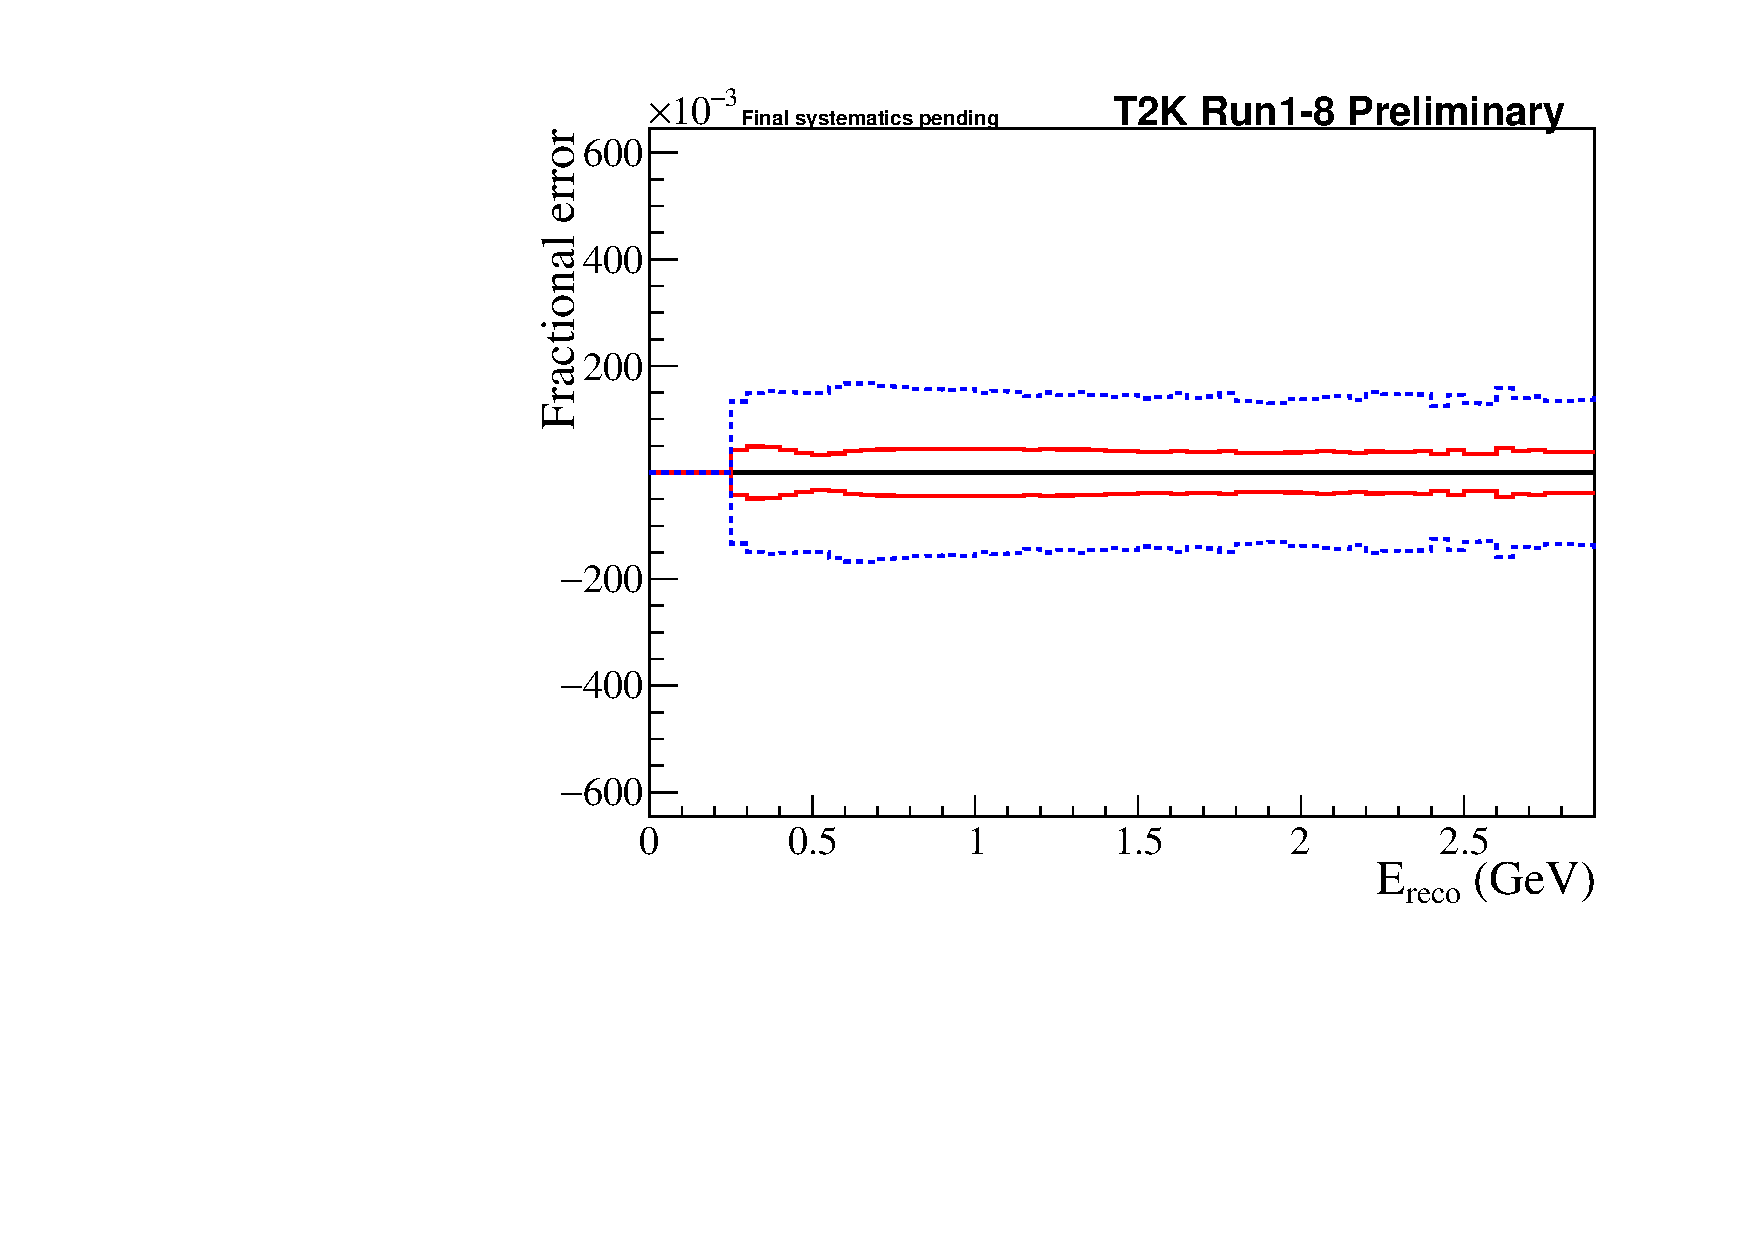
\includegraphics[width=0.9\textwidth]{systematics/envelopes/sk_errors/sk_error_table_1Rmu_banff_constrained_envelope_fractional}
		\caption{Muon-like, neutrino mode}
	\end{subfigure}
	\begin{subfigure}[b]{0.49\textwidth}
		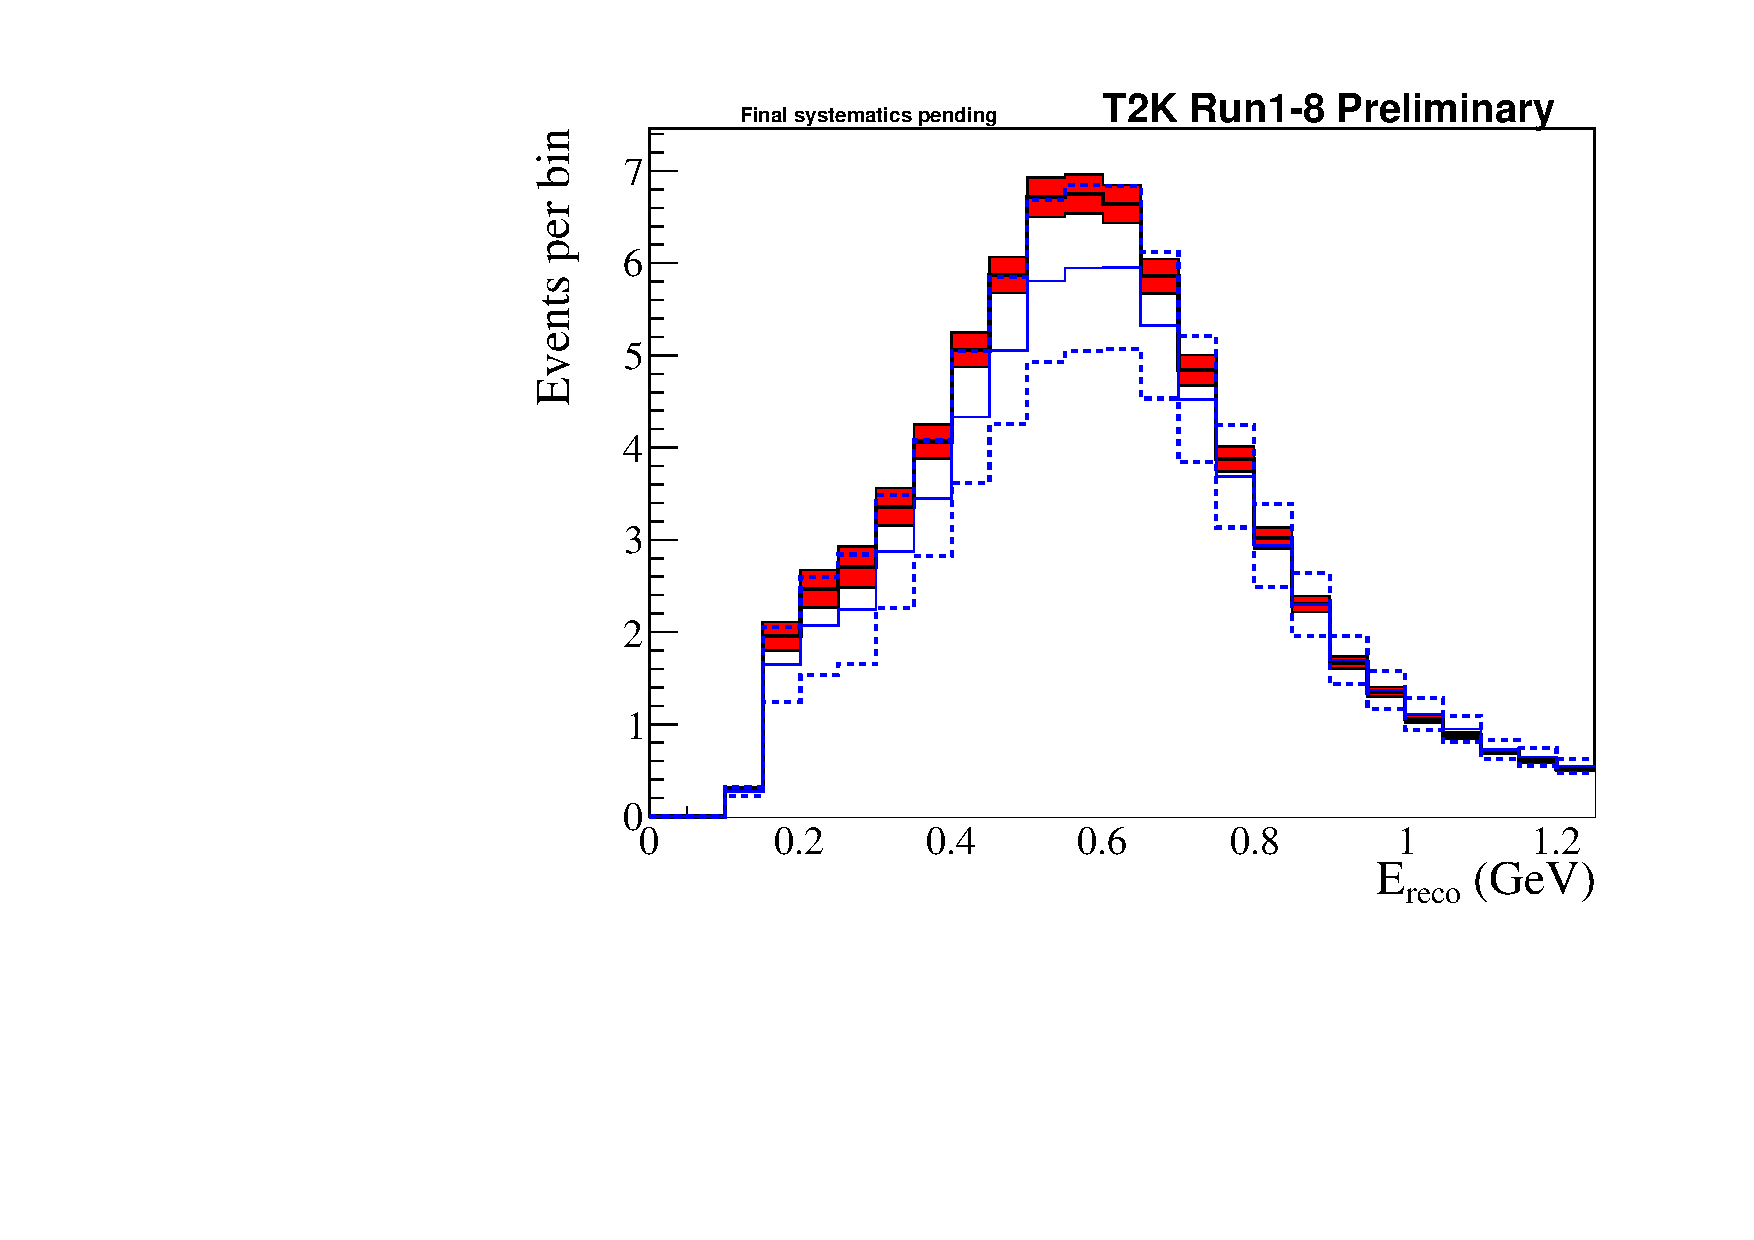
\includegraphics[width=0.9\textwidth]{systematics/envelopes/sk_errors/sk_error_table_1Re_banff_constrained_envelope}
		\caption{Electron-like, neutrino mode}
	\end{subfigure}
	\begin{subfigure}[b]{0.49\textwidth}
		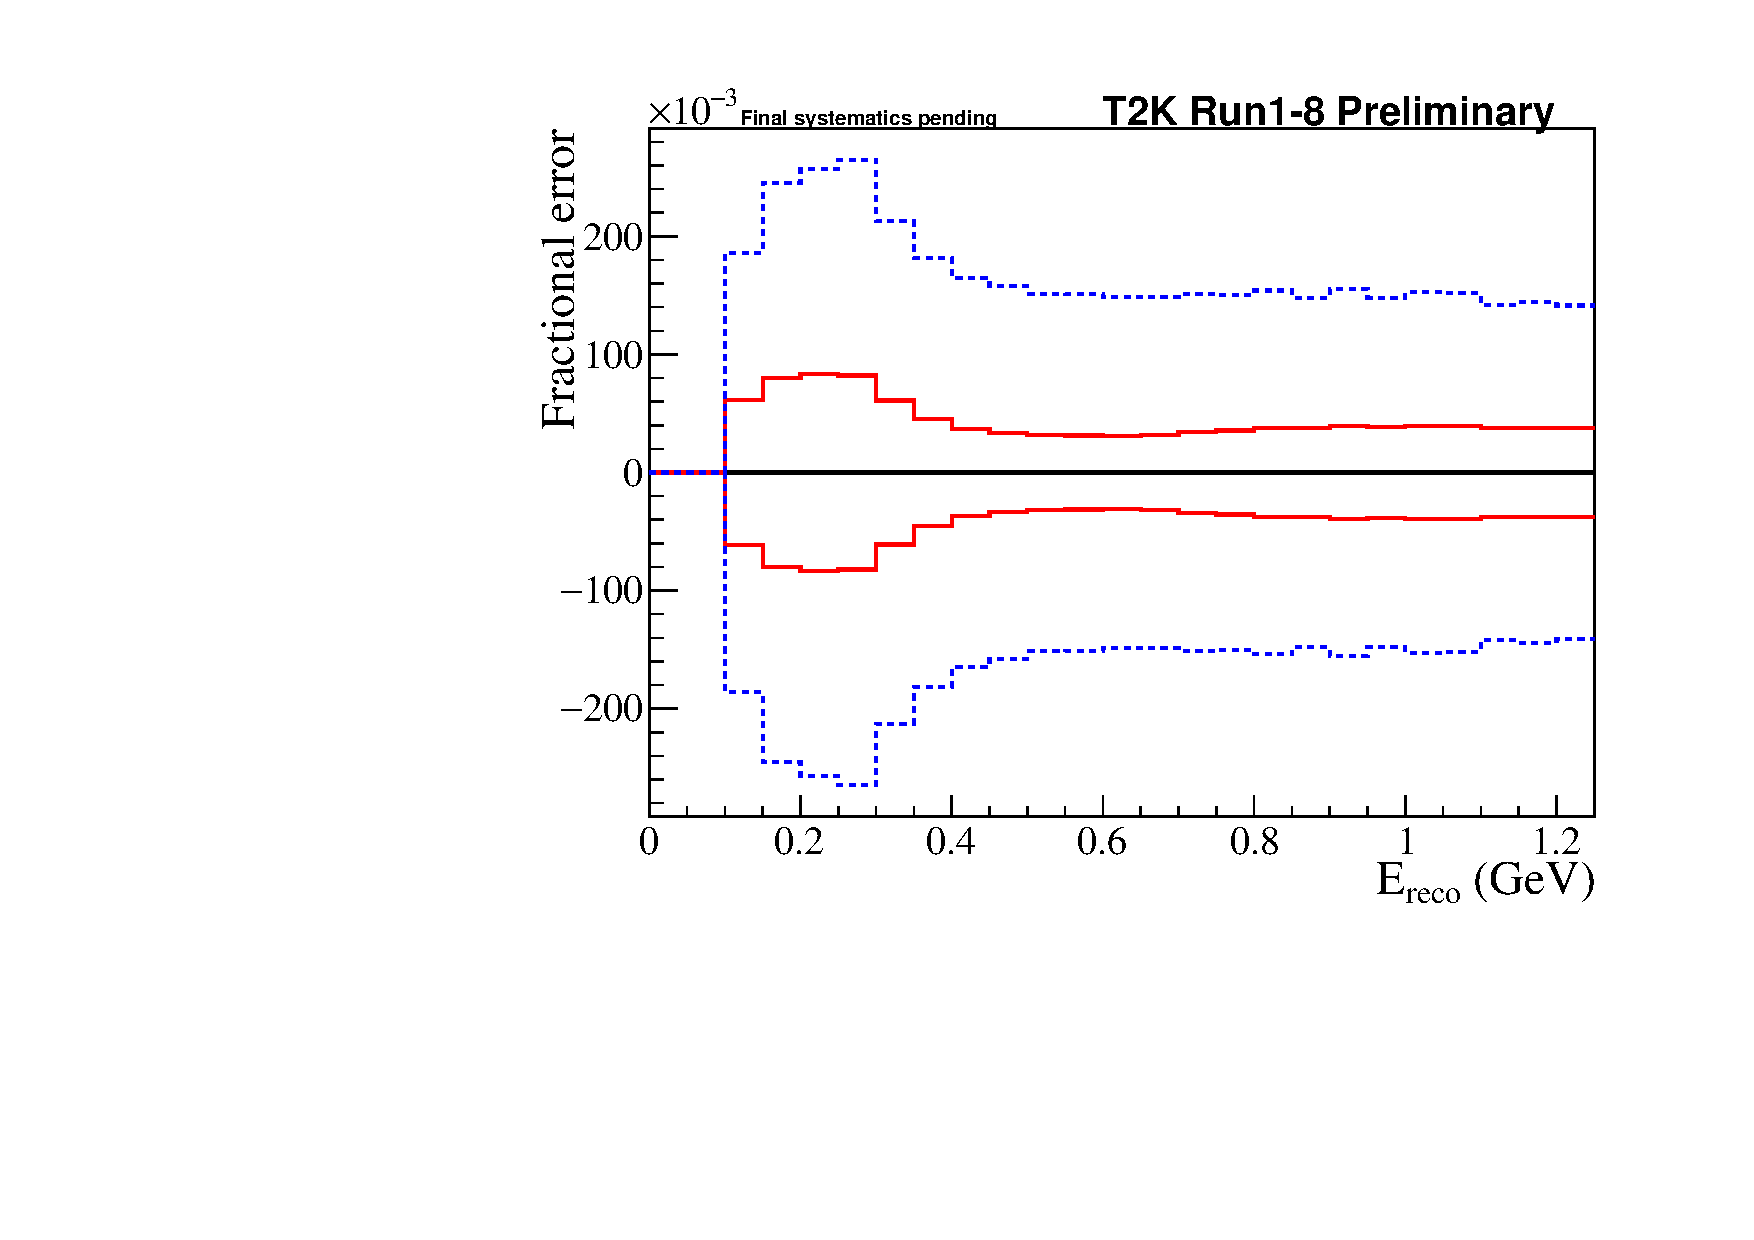
\includegraphics[width=0.9\textwidth]{systematics/envelopes/sk_errors/sk_error_table_1Re_banff_constrained_envelope_fractional}
		\caption{Electron-like, neutrino mode}
	\end{subfigure}
	\begin{subfigure}[b]{0.49\textwidth}
		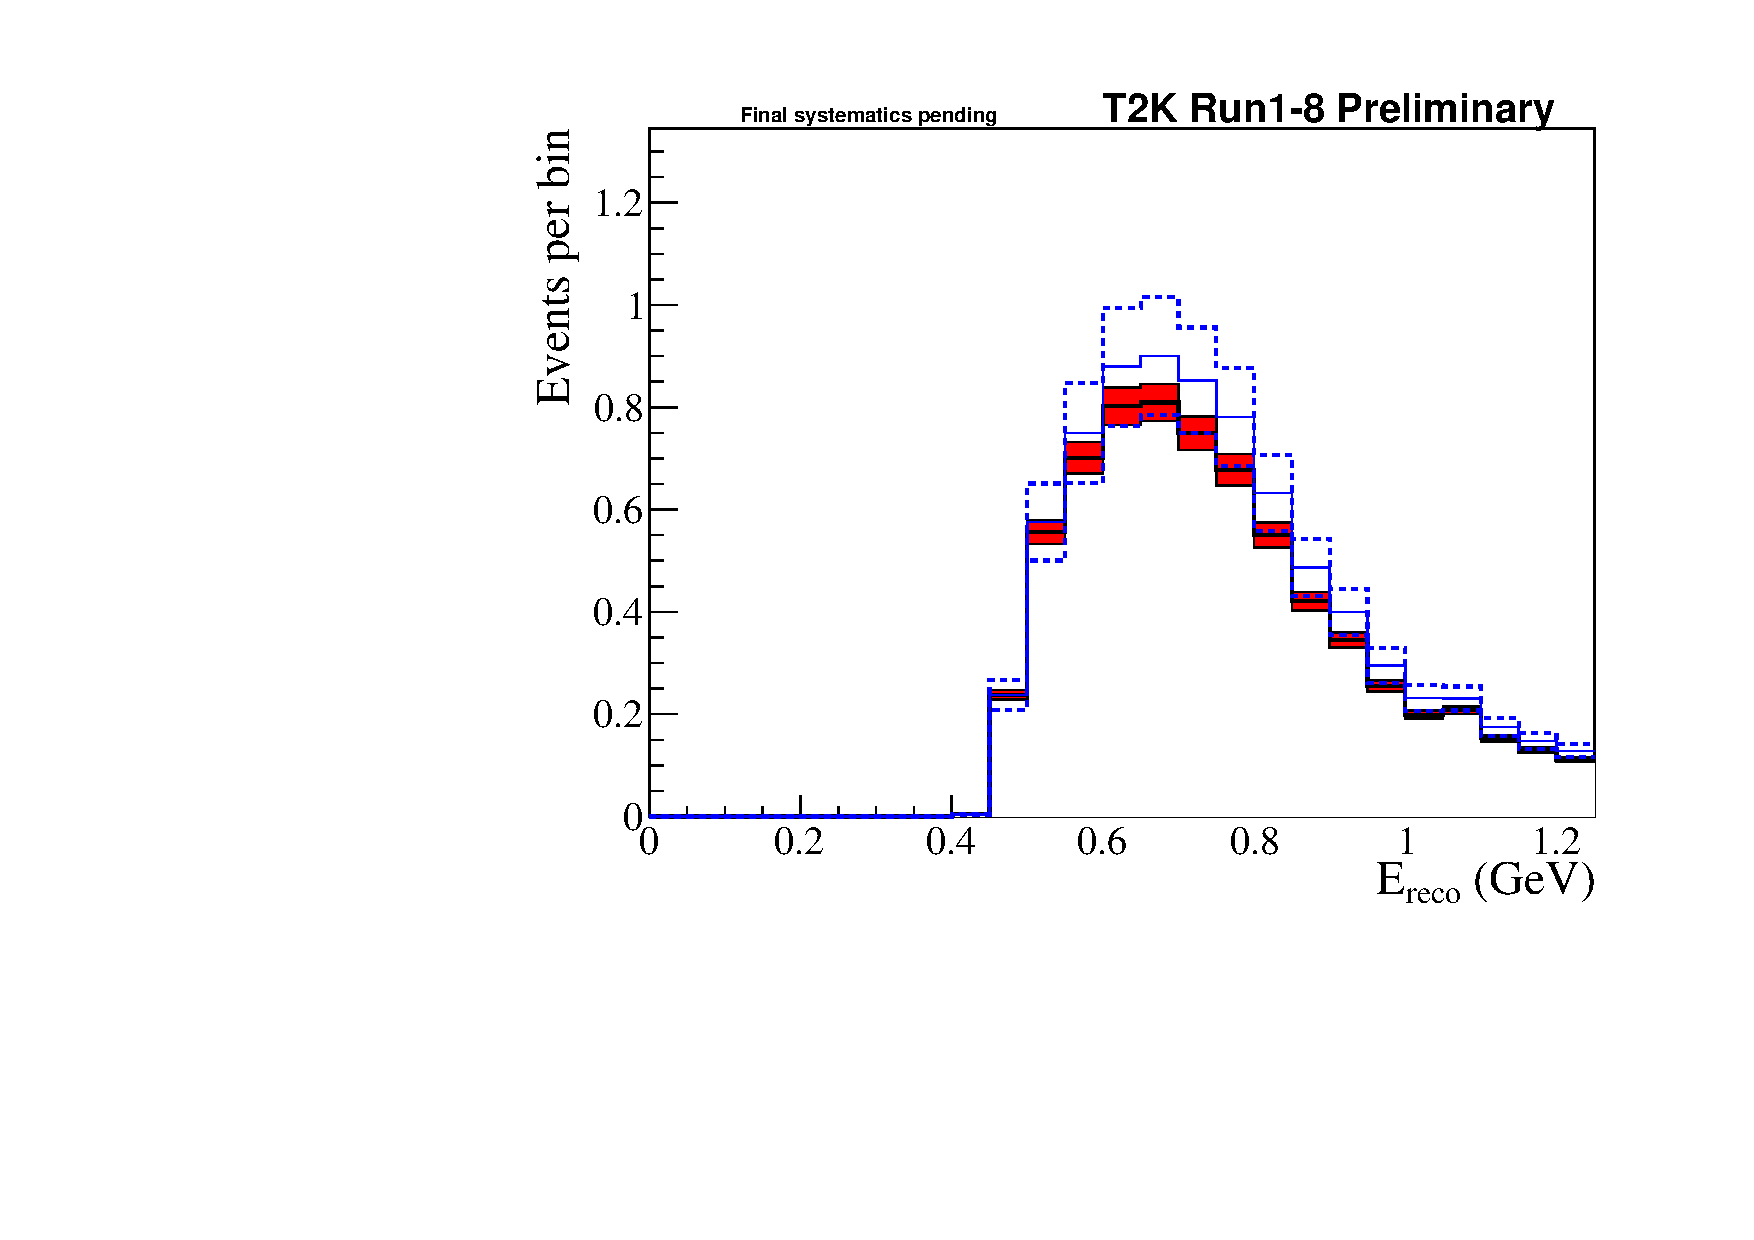
\includegraphics[width=0.9\textwidth]{systematics/envelopes/sk_errors/sk_error_table_MultiRe_banff_constrained_envelope}
		\caption{\nueCConepi-like, neutrino mode}
	\end{subfigure}
	\begin{subfigure}[b]{0.49\textwidth}
		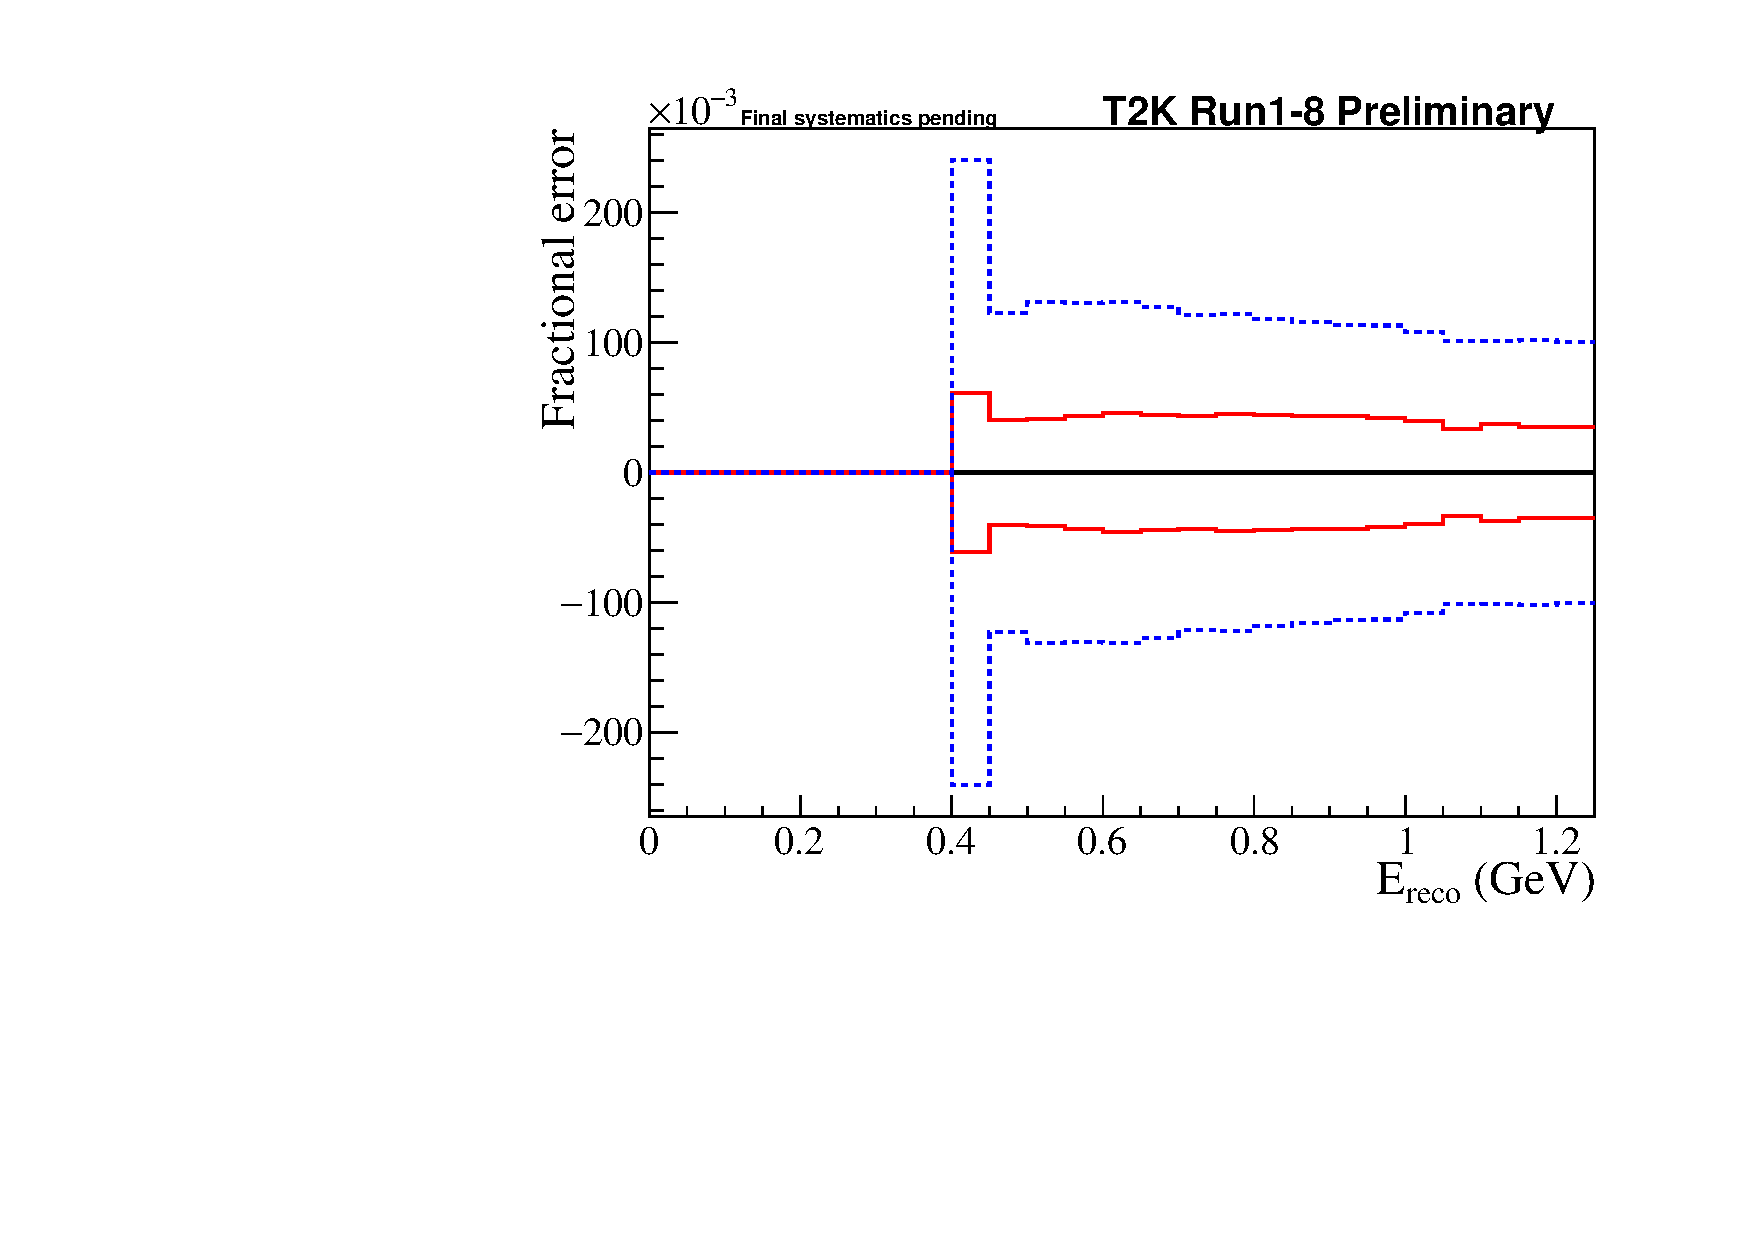
\includegraphics[width=0.9\textwidth]{systematics/envelopes/sk_errors/sk_error_table_MultiRe_banff_constrained_envelope_fractional}
		\caption{\nueCConepi-like, neutrino mode}
	\end{subfigure}
	\caption {
		Error envelopes (left) and fractional errors (right) for the reconstructed neutrino energy spectrum for the flux and constrained cross-section systematic parameters for pre-BANFF (blue) and post-BANFF (red) errors. \num{1e4} toys are generated for the Asimov data set A with randomized systematic parameters with correlations taken into account.
	}
	\label{fig:sk_envelopes_banff}
\end{figure*}
\clearpage

\begin{figure*}
	\center
	\begin{subfigure}[b]{0.49\textwidth}
		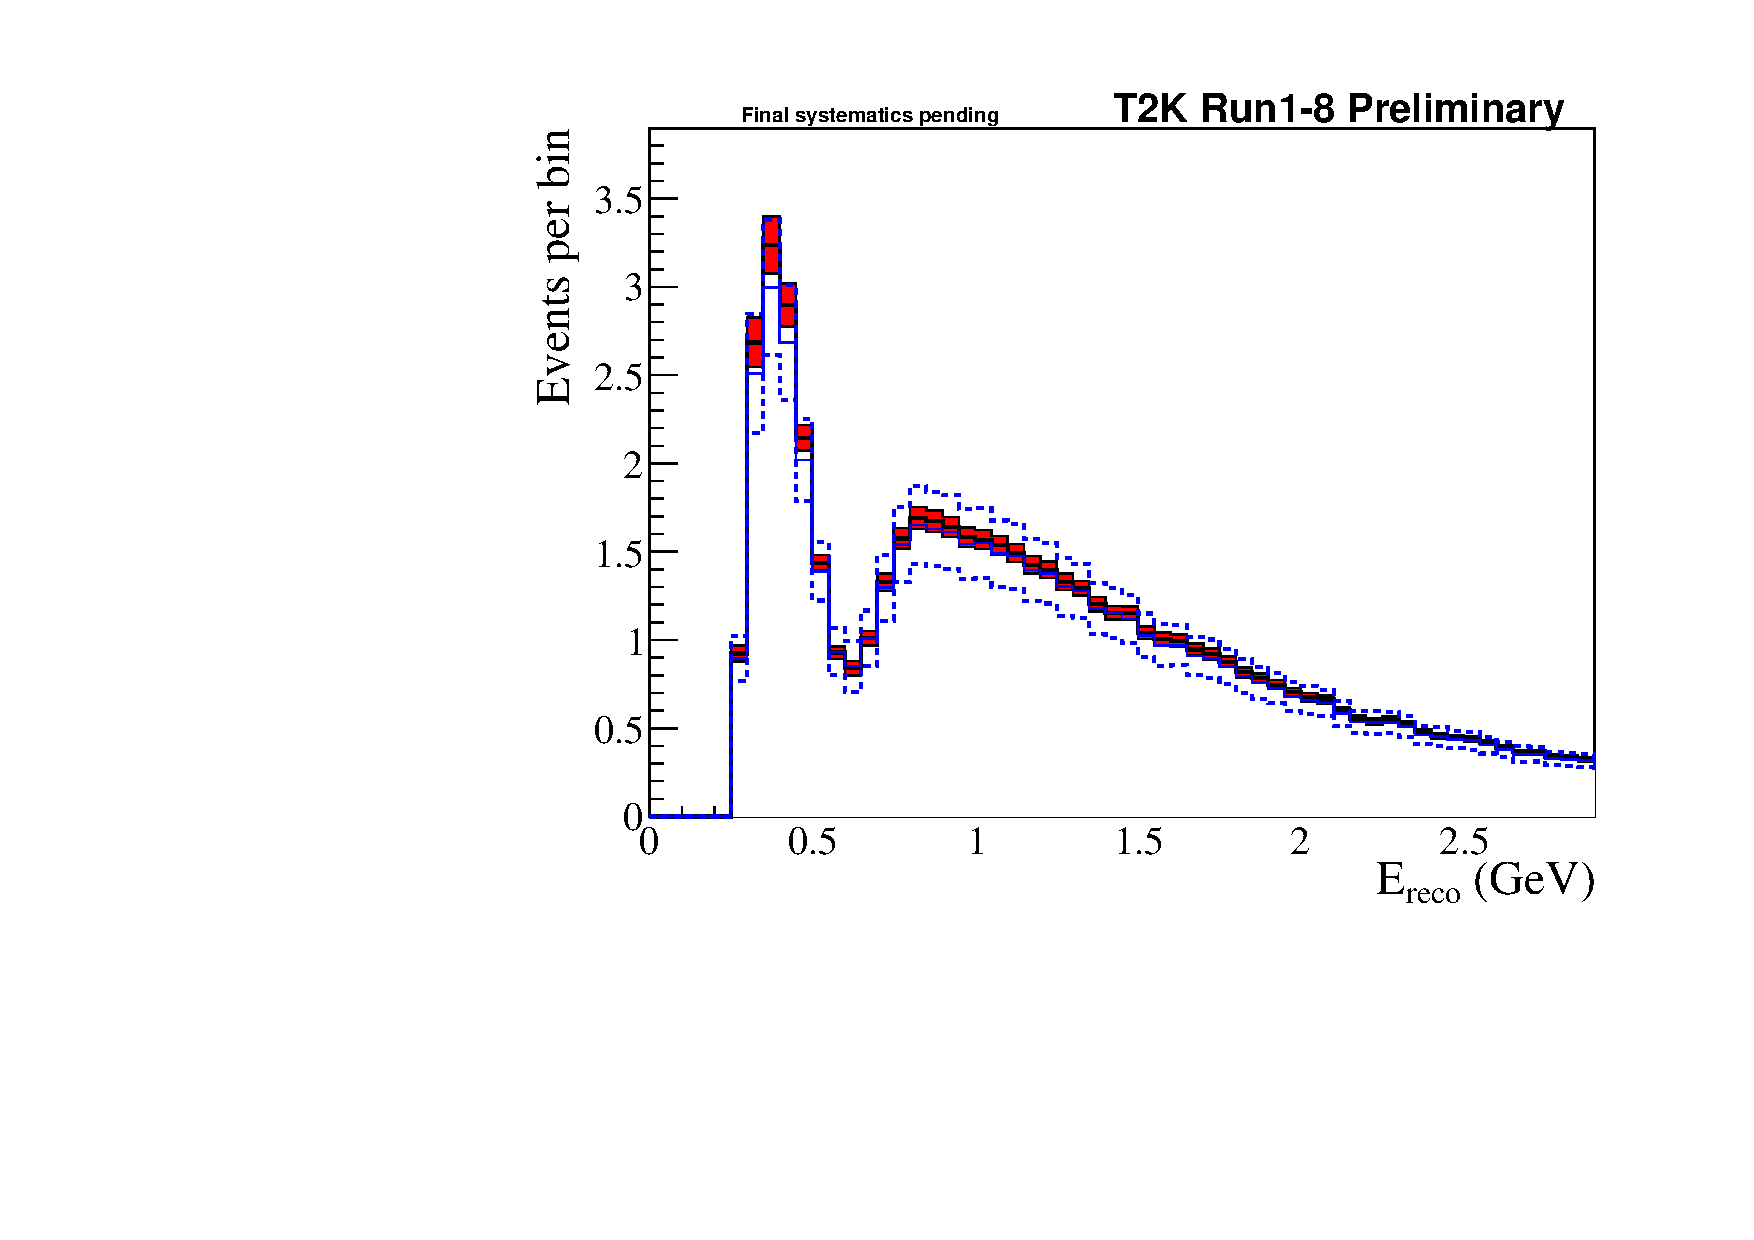
\includegraphics[width=0.9\textwidth]{systematics/envelopes/sk_errors/sk_error_table_RHC1Rmu_banff_constrained_envelope}
		\caption{Muon-like, antineutrino mode}
	\end{subfigure}
	\begin{subfigure}[b]{0.49\textwidth}
		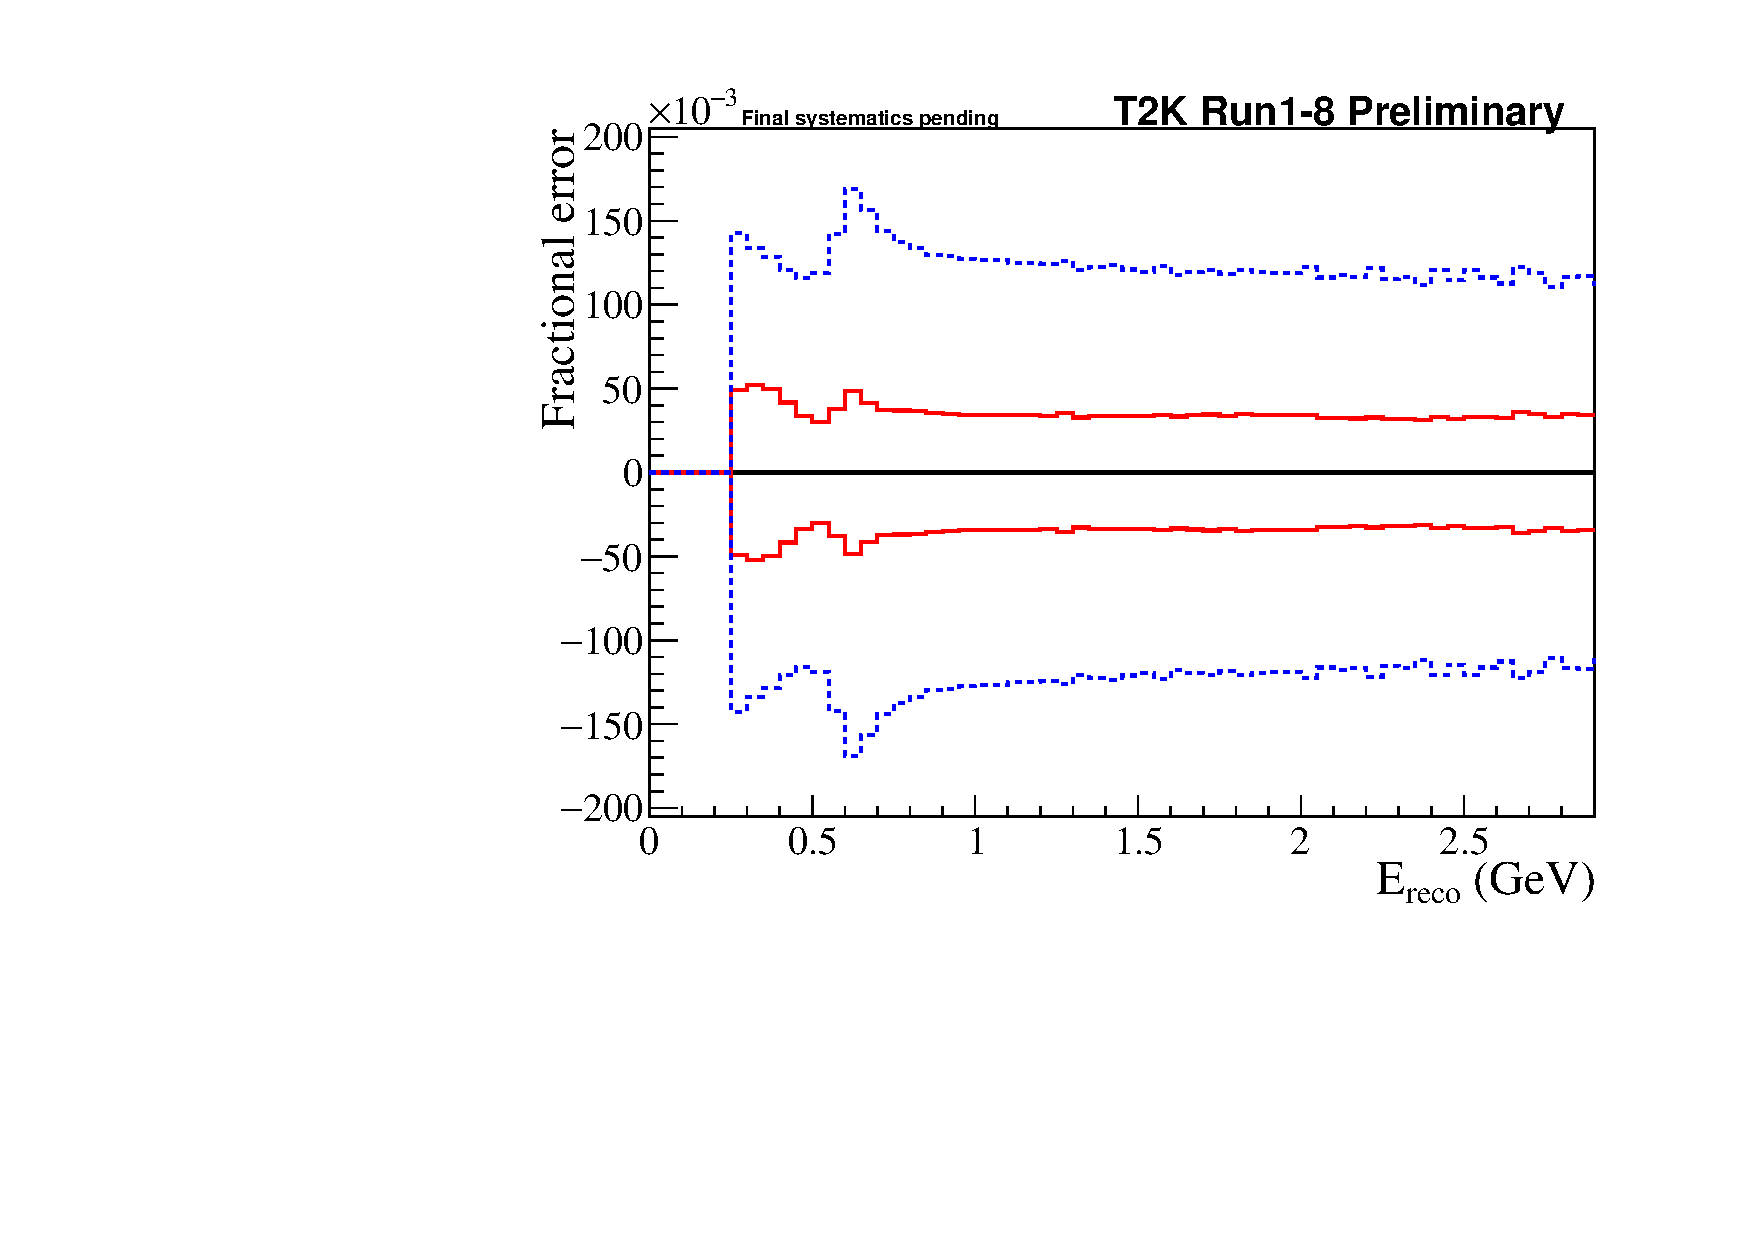
\includegraphics[width=0.9\textwidth]{systematics/envelopes/sk_errors/sk_error_table_RHC1Rmu_banff_constrained_envelope_fractional}
		\caption{Muon-like, antineutrino mode}
	\end{subfigure}
	\begin{subfigure}[b]{0.49\textwidth}
		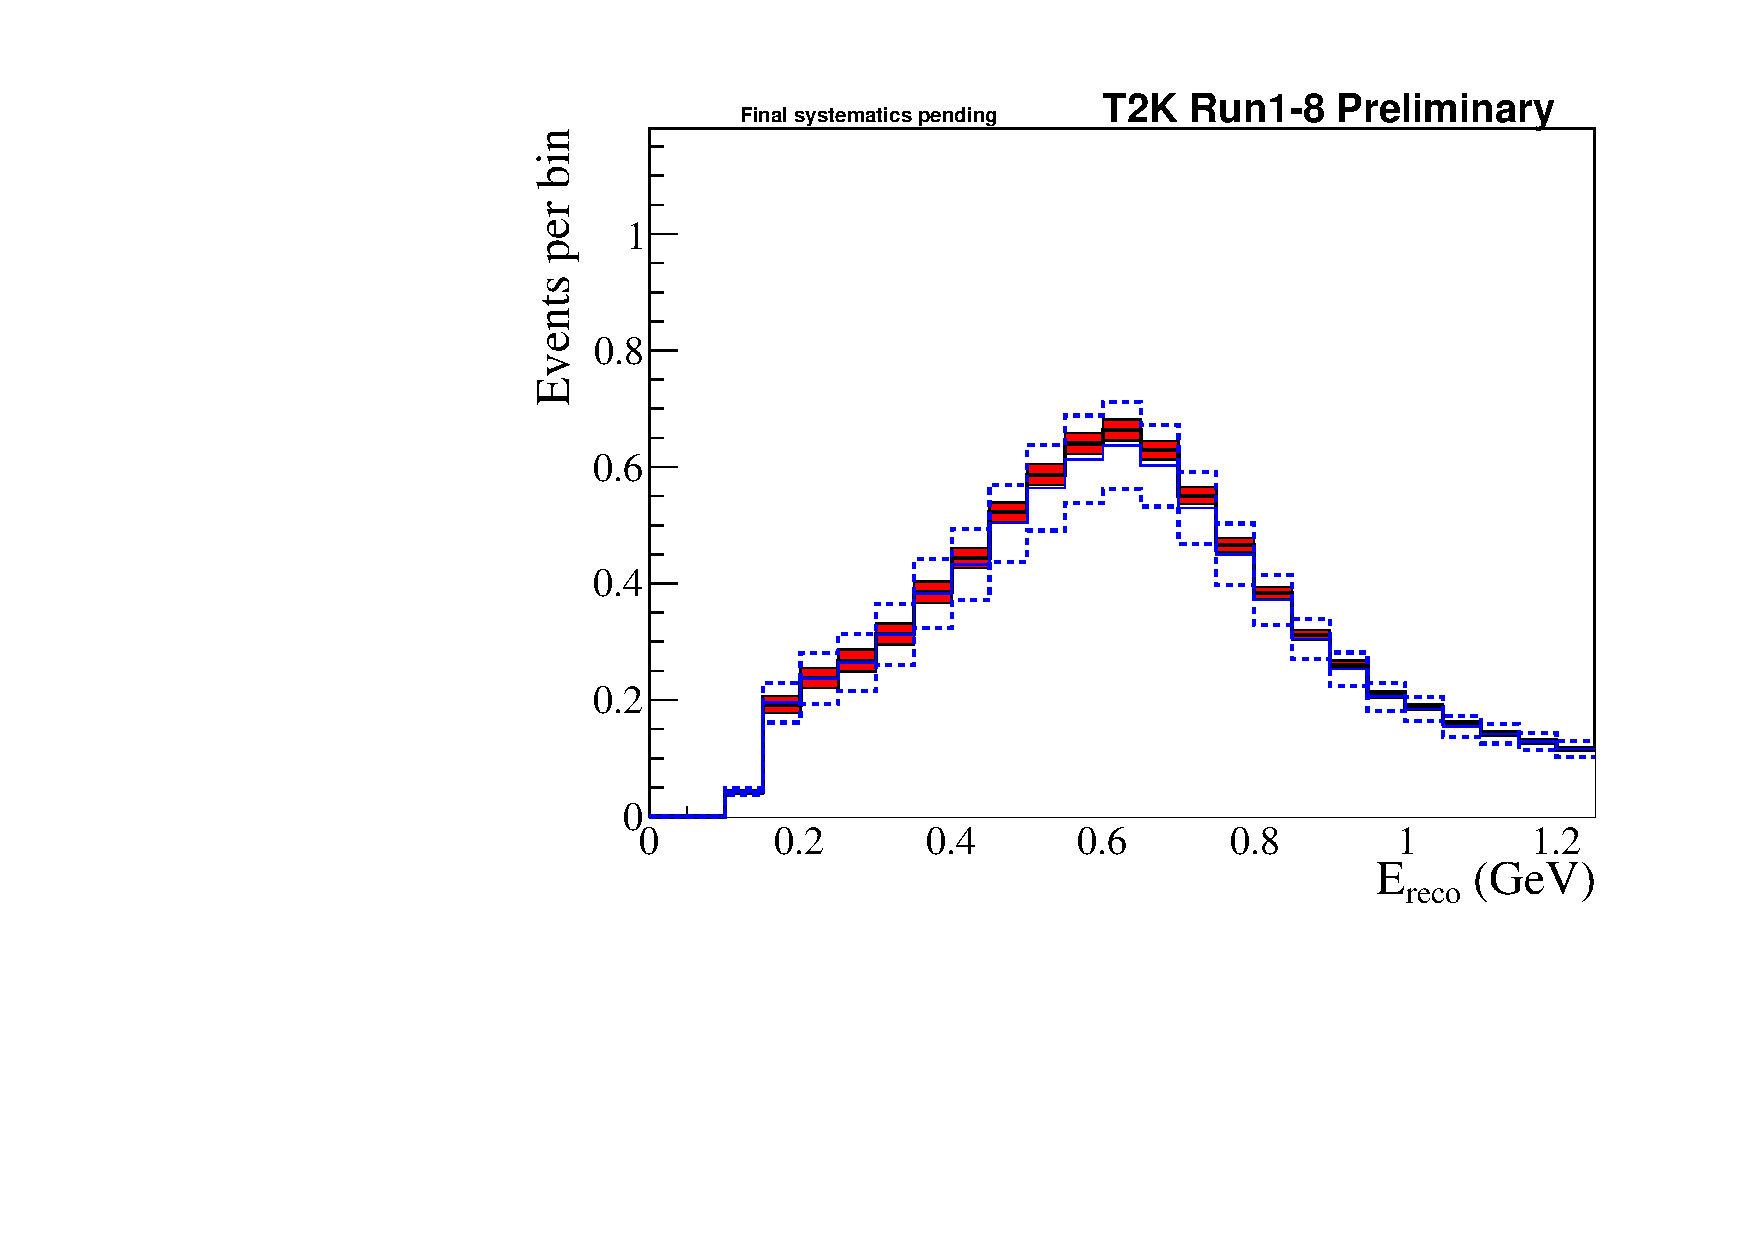
\includegraphics[width=0.9\textwidth]{systematics/envelopes/sk_errors/sk_error_table_RHC1Re_banff_constrained_envelope}
		\caption{Electron-like antineutrino mode}
	\end{subfigure}
	\begin{subfigure}[b]{0.49\textwidth}
		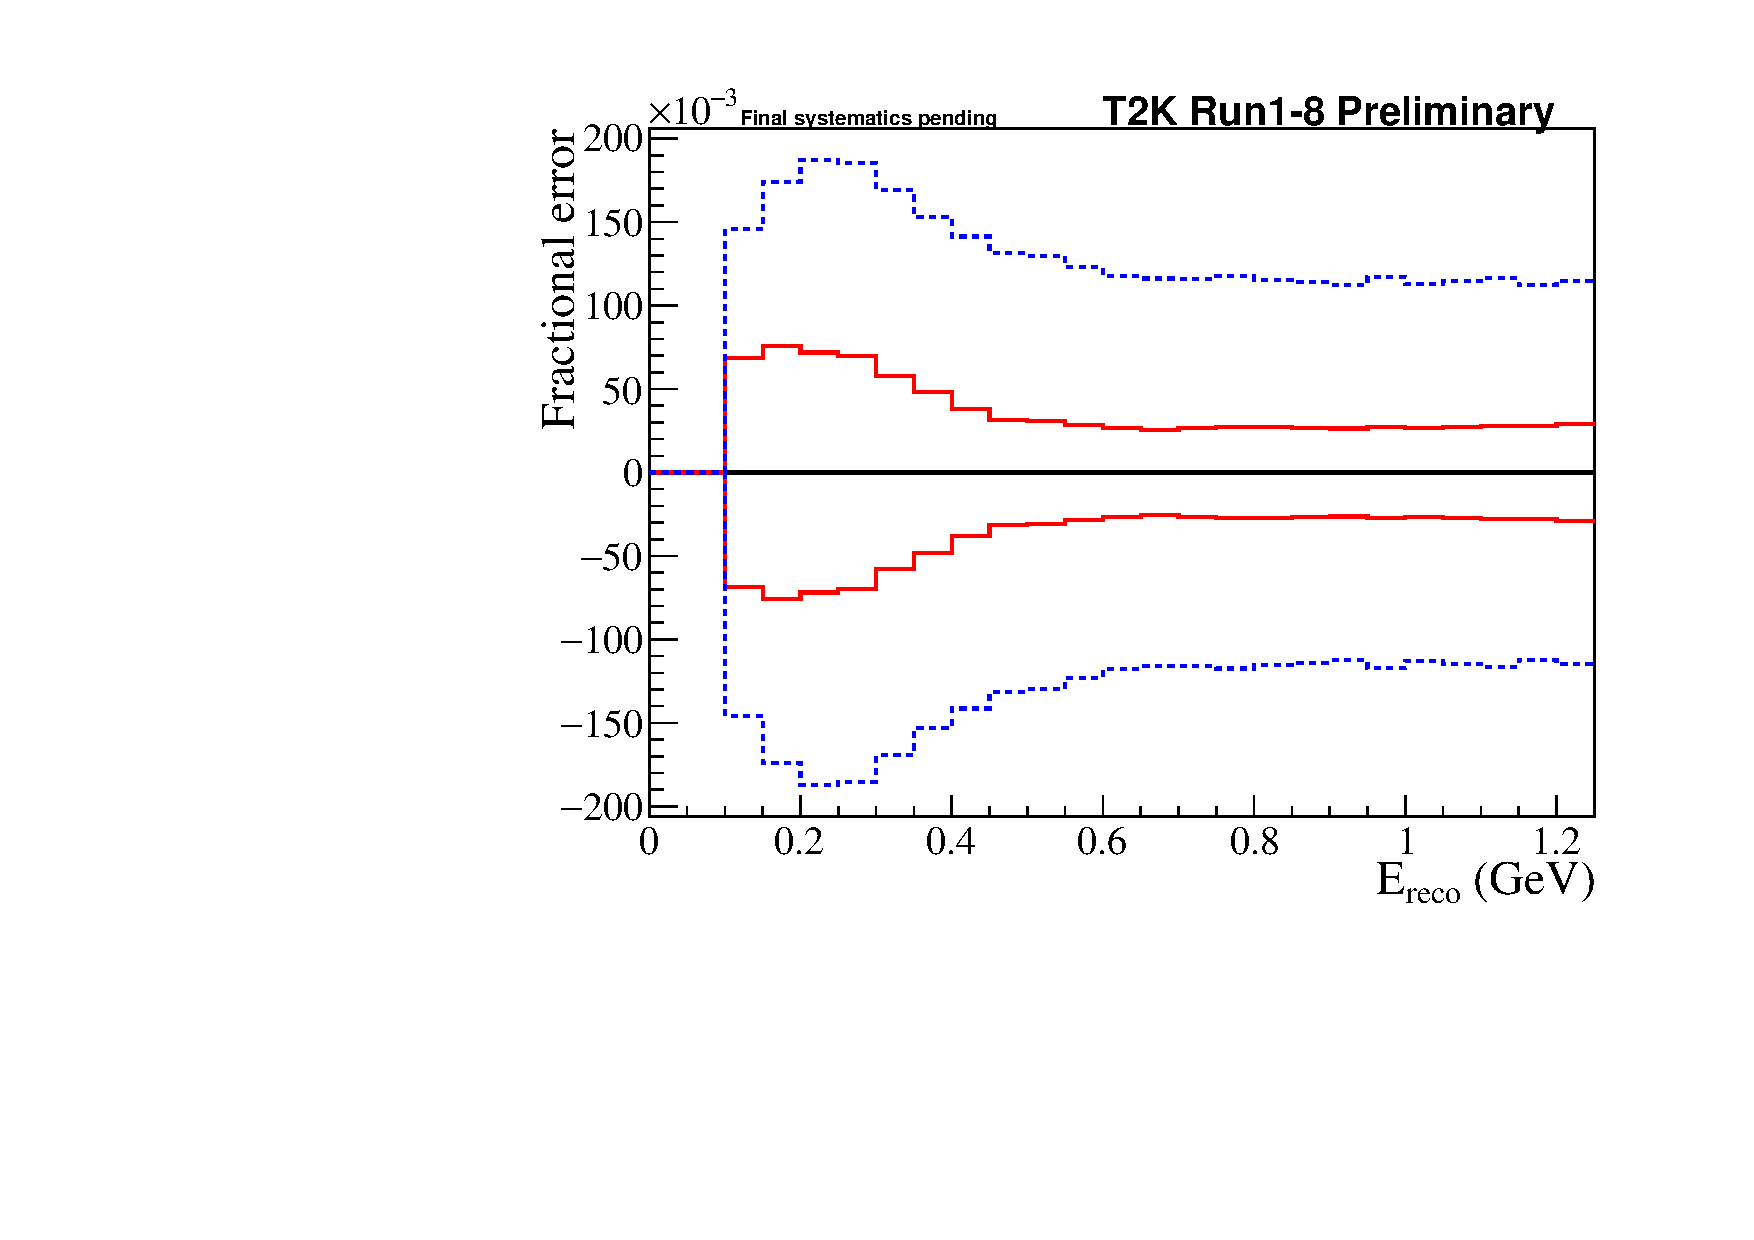
\includegraphics[width=0.9\textwidth]{systematics/envelopes/sk_errors/sk_error_table_RHC1Re_banff_constrained_envelope_fractional}
		\caption{Electron-like antineutrino mode}
	\end{subfigure}
	\caption {
		Error envelopes (left) and fractional error (right) for the reconstructed neutrino energy spectrum for the flux and constrained cross-section systematic parameters for pre-BANFF (blue) and post-BANFF (red) errors. \num{1e4} toys are generated for the Asimov data set A with randomized systematic parameters with correlations taken into account.
	}
	\label{fig:sk_envelopes_banff_b}
\end{figure*}
\clearpage